\documentclass[12pt,fleqn]{article}\usepackage[]{graphicx}\usepackage[]{color}
%% maxwidth is the original width if it is less than linewidth
%% otherwise use linewidth (to make sure the graphics do not exceed the margin)
\makeatletter
\def\maxwidth{ %
  \ifdim\Gin@nat@width>\linewidth
    \linewidth
  \else
    \Gin@nat@width
  \fi
}
\makeatother

\definecolor{fgcolor}{rgb}{0.345, 0.345, 0.345}
\newcommand{\hlnum}[1]{\textcolor[rgb]{0.686,0.059,0.569}{#1}}%
\newcommand{\hlstr}[1]{\textcolor[rgb]{0.192,0.494,0.8}{#1}}%
\newcommand{\hlcom}[1]{\textcolor[rgb]{0.678,0.584,0.686}{\textit{#1}}}%
\newcommand{\hlopt}[1]{\textcolor[rgb]{0,0,0}{#1}}%
\newcommand{\hlstd}[1]{\textcolor[rgb]{0.345,0.345,0.345}{#1}}%
\newcommand{\hlkwa}[1]{\textcolor[rgb]{0.161,0.373,0.58}{\textbf{#1}}}%
\newcommand{\hlkwb}[1]{\textcolor[rgb]{0.69,0.353,0.396}{#1}}%
\newcommand{\hlkwc}[1]{\textcolor[rgb]{0.333,0.667,0.333}{#1}}%
\newcommand{\hlkwd}[1]{\textcolor[rgb]{0.737,0.353,0.396}{\textbf{#1}}}%
\let\hlipl\hlkwb

\usepackage{framed}
\makeatletter
\newenvironment{kframe}{%
 \def\at@end@of@kframe{}%
 \ifinner\ifhmode%
  \def\at@end@of@kframe{\end{minipage}}%
  \begin{minipage}{\columnwidth}%
 \fi\fi%
 \def\FrameCommand##1{\hskip\@totalleftmargin \hskip-\fboxsep
 \colorbox{shadecolor}{##1}\hskip-\fboxsep
     % There is no \\@totalrightmargin, so:
     \hskip-\linewidth \hskip-\@totalleftmargin \hskip\columnwidth}%
 \MakeFramed {\advance\hsize-\width
   \@totalleftmargin\z@ \linewidth\hsize
   \@setminipage}}%
 {\par\unskip\endMakeFramed%
 \at@end@of@kframe}
\makeatother

\definecolor{shadecolor}{rgb}{.97, .97, .97}
\definecolor{messagecolor}{rgb}{0, 0, 0}
\definecolor{warningcolor}{rgb}{1, 0, 1}
\definecolor{errorcolor}{rgb}{1, 0, 0}
\newenvironment{knitrout}{}{} % an empty environment to be redefined in TeX

\usepackage{alltt}
\usepackage{pgfplots}
\pgfplotsset{compat=1.7}
\usepackage[margin=1in]{geometry}
\usepackage{amsmath,amsthm,amssymb,scrextend}
\usepackage{fancyhdr}
\pagestyle{fancy}
\DeclareMathOperator{\rng}{Rng}
\DeclareMathOperator{\dom}{Dom}
\newcommand{\R}{\mathbb R}
\newcommand{\cont}{\subseteq}
\newcommand{\N}{\mathbb N}
\newcommand{\Z}{\mathbb Z}
\usepackage{tikz}
\usepackage{pgfplots}
\usepackage{amsmath}
\usepackage[mathscr]{euscript}
\let\euscr\mathscr \let\mathscr\relax% just so we can load this and rsfs
\usepackage[scr]{rsfso}
\usepackage{amsthm}
\usepackage{amssymb}
\usepackage{multicol}
\usepackage[colorlinks=true, pdfstartview=FitV, linkcolor=blue,
citecolor=blue, urlcolor=blue]{hyperref}

\DeclareMathOperator{\arcsec}{arcsec}
\DeclareMathOperator{\arccot}{arccot}
\DeclareMathOperator{\arccsc}{arccsc}
\newcommand{\ddx}{\frac{d}{dx}}
\newcommand{\dfdx}{\frac{df}{dx}}
\newcommand{\ddxp}[1]{\frac{d}{dx}\left( #1 \right)}
\newcommand{\dydx}{\frac{dy}{dx}}
\let\ds\displaystyle
\newcommand{\intx}[1]{\int #1 \, dx}
\newcommand{\intt}[1]{\int #1 \, dt}
\newcommand{\defint}[3]{\int_{#1}^{#2} #3 \, dx}
\newcommand{\imp}{\Rightarrow}
\newcommand{\un}{\cup}
\newcommand{\inter}{\cap}
\newcommand{\ps}{\mathscr{P}}
\newcommand{\set}[1]{\left\{ #1 \right\}}

\usepackage{enumerate} % enable \begin{enumerate}[1.]
\renewcommand{\labelenumi}{\alph{enumi}.} %first level: (a),(b)
\renewcommand{\labelenumii}{\roman{enumii}.} %second level: i,ii

\theoremstyle{definition}
\newtheorem*{sol}{Solution}
\newtheorem*{claim}{Claim}
\newtheorem{problem}{}
% ---------------------------------------------------------------------------------------------
\IfFileExists{upquote.sty}{\usepackage{upquote}}{}
\begin{document}
\lhead{Machine Learning}
\chead{Zhijian Liu}
\rhead{\today}



% Just put your proofs in between the \begin{proof} and the \end{proof} statements!

\section*{Homework \# 11: Support Vector Machines (Chap. 9)}
	\begin{enumerate}[1.]
	% 1.
	  \item \textbf{(Chap. 9, \# 1a, p. 368)} This problem involves a hyperplane in two dimensions. Sketch the hyperplane $1+3 X_{1}-X_{2}=0$. Indicate the set of points for which $1+3 X_{1}-X_{2}>0$, as well as the set of points for which $1+3 X_{1}-X_{2}<0$.\\
\begin{knitrout}
\definecolor{shadecolor}{rgb}{0.969, 0.969, 0.969}\color{fgcolor}

{\centering \includegraphics[width=0.5\linewidth]{figure/1-1} 

}



\end{knitrout}
    For the points which $1+3 X_{1}-X_{2}<0$, they are colored red. For the points which $1+3 X_{1}-X_{2}>0$, they are colored blue.
  % 2.
    \item \textbf{(Chap. 9, \# 2, p. 368)} We have seen that in p = 2 dimensions, a linear decision boundary takes the form $\beta_{0}+\beta_{1} X_{1}+\beta_{2} X_{2}=0$. We now investigate a \textbf{non-linear} decision boundary.
        \begin{enumerate}[(a)]
        % (a)
          \item Sketch the curve $\left(1+X_{1}\right)^{2}+\left(2-X_{2}\right)^{2}=4$.\\
\begin{knitrout}
\definecolor{shadecolor}{rgb}{0.969, 0.969, 0.969}\color{fgcolor}

{\centering \includegraphics[width=0.6\linewidth]{figure/2_a-1} 

}



\end{knitrout}

        % (b)
          \item On your sketch, indicate the set of points for which $\left(1+X_{1}\right)^{2}+\left(2-X_{2}\right)^{2}>4$, as well as the set of points for which $\left(1+X_{1}\right)^{2}+\left(2-X_{2}\right)^{2} \leq 4$.\\
\begin{knitrout}
\definecolor{shadecolor}{rgb}{0.969, 0.969, 0.969}\color{fgcolor}

{\centering \includegraphics[width=0.6\linewidth]{figure/2_b-1} 

}



\end{knitrout}
        Blue points indicate $\left(1+X_{1}\right)^{2}+\left(2-X_{2}\right)^{2}>4$, while red points indicate $\left(1+X_{1}\right)^{2}+\left(2-X_{2}\right)^{2} \leq 4$.
        % (c)
          \item Suppose that a classifier assigns an observation to the blue class if $\left(1+X_{1}\right)^{2}+\left(2-X_{2}\right)^{2}>4$, and to the red class otherwise. To what class is the observation (0, 0) classified? (-1, 1)? (2,2)? (3,8)?\\
\begin{knitrout}
\definecolor{shadecolor}{rgb}{0.969, 0.969, 0.969}\color{fgcolor}

{\centering \includegraphics[width=0.6\linewidth,height=0.8\linewidth]{figure/2_c-1} 

}



\end{knitrout}
          The observation (0, 0), (2,2), (3,8) are classified as blue while (-1, 1) is classified as red.
        % (d)
          \item Argue that while the decision boundary in (c) is not linear in terms of $X_1$ and $X_2$, it is linear in terms of $X_1$, $X_1^2$, $X_2$, and $X_2^2$.
          \begin{align*}
              &\left(1+X_{1}\right)^{2}+\left(2-X_{2}\right)^{2}\\
            = &1 + 2X_{1} + X_{1}^2 + 4 - 4X_{2} + X_{2}^2\\
            = &5 + 2X_{1} + X_{1}^2 + 4 - 4X_{2} + X_{2}^2
          \end{align*}
        \end{enumerate}
  % 3.
    \item \textbf{(Chap. 9, \# 3, p. 368)} Here we explore the maximal margin classifier on a toy data set.
        \begin{enumerate}[(a)]
        % a.
          \item We are given $n = 7$ observations in $p = 2$ dimensions. For each observation, there is an associated class label.\\
            \begin{center}
              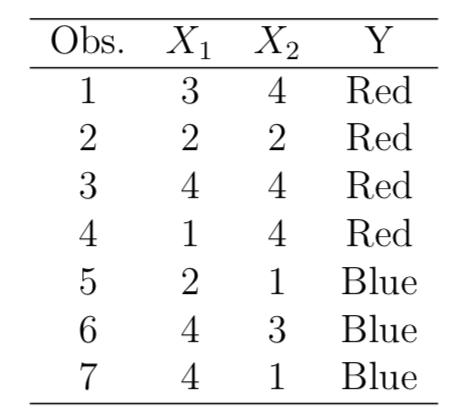
\includegraphics[scale=0.65]{table}
            \end{center}
            Sketch the observations.\\
\begin{knitrout}
\definecolor{shadecolor}{rgb}{0.969, 0.969, 0.969}\color{fgcolor}

{\centering \includegraphics[width=0.8\linewidth]{figure/3_a-1} 

}



\end{knitrout}

        % b.
          \item Sketch the optimal separating hyperplane, and provide the equation for this hyperplane such as in exercise \#1.\\
\begin{knitrout}
\definecolor{shadecolor}{rgb}{0.969, 0.969, 0.969}\color{fgcolor}

{\centering \includegraphics[width=0.8\linewidth]{figure/3_b-1} 

}



\end{knitrout}

        % c.
          \item Describe the classification rule for the maximal margin classifier. It should be something along the lines of "Classify to Red if $\beta_{0}+\beta_{1} X_{1}+\beta_{2} X_{2}>0$, and classify to Blue otherwise". Provide the values for $beta_0$, $beta_1$, and $beta_2$.\\
          The observation is classified to Red if $0.5 - X_{1} + X_{2}>0$, and classified to Blue otherwise. $beta_0 = 0.5$, $beta_1 = -1$, and $beta_2 = 1$.
        % d.
          \item On your sketch, indicate the margin for the maximal margin hyperplane.\\
          Maximal margin: $M=\frac{\sqrt{0.5^2+0.5^2}}{2}=\frac{\sqrt{2}}{4}$.
        % e.
          \item Indicate the support vectors for the maximal margin classifier.\\
\begin{knitrout}
\definecolor{shadecolor}{rgb}{0.969, 0.969, 0.969}\color{fgcolor}

{\centering \includegraphics[width=0.8\linewidth]{figure/3_e-1} 

}



\end{knitrout}
        The points (2,1), (2,2), (4,3) and (4,4) are the support vectors.
        % f.
          \item Argue that a slight movement of the seventh observation would not affect the maximal margin hyperplane.
\begin{knitrout}
\definecolor{shadecolor}{rgb}{0.969, 0.969, 0.969}\color{fgcolor}

{\centering \includegraphics[width=0.8\linewidth]{figure/3_f-1} 

}



\end{knitrout}
        For the seventh observation, (4,1), a slight movement would not affect the maximal margin hyperplane as long as it does not enter the existed hyperplane.
        % g.
          \item Sketch a hyperplane that is not the optimal separating hyperplane, and provide the equation for this hyperplane.
\begin{knitrout}
\definecolor{shadecolor}{rgb}{0.969, 0.969, 0.969}\color{fgcolor}

{\centering \includegraphics[width=0.8\linewidth]{figure/3_g-1} 

}



\end{knitrout}
        This hyperplane is not optimal since it does not generate the largest margin, and the equation for this hyperplane is $0.3 - 0.9X_{1} + X_{2}=0$
        % h.
          \item Draw an additional observation on the plot so that the two classes are no longer separable by a hyperplane.
\begin{knitrout}
\definecolor{shadecolor}{rgb}{0.969, 0.969, 0.969}\color{fgcolor}

{\centering \includegraphics[width=0.8\linewidth]{figure/3_h-1} 

}



\end{knitrout}

        \end{enumerate}
  % 4.
    \item \textbf{(Chap. 9, \# 7, p. 371)} In this problem, you will use support vector approaches in order to predict whether a given car gets high or low gas mileage based on the Auto data set (from \texttt{ISLR}).
      \begin{enumerate}
      % a.
        \item Create a binary variable that takes on a 1 for cars with gas mileage above the median, and a 0 for cars with gas mileage below the median.
\begin{knitrout}
\definecolor{shadecolor}{rgb}{0.969, 0.969, 0.969}\color{fgcolor}\begin{kframe}
\begin{alltt}
\hlstd{Auto}\hlopt{$}\hlstd{mileage} \hlkwb{<-} \hlkwd{rep}\hlstd{(}\hlnum{1}\hlstd{,}\hlkwd{nrow}\hlstd{(Auto))}
\hlstd{Auto}\hlopt{$}\hlstd{mileage[Auto}\hlopt{$}\hlstd{mpg} \hlopt{<} \hlkwd{median}\hlstd{(Auto}\hlopt{$}\hlstd{mpg)]} \hlkwb{<-} \hlnum{0}
\hlstd{Auto}\hlopt{$}\hlstd{mileage} \hlkwb{<-} \hlkwd{as.factor}\hlstd{(Auto}\hlopt{$}\hlstd{mileage)}
\end{alltt}
\end{kframe}
\end{knitrout}

      % b.
        \item Fit a support vector classifier to the data with various values of cost, in order to predict whether a car gets high or low gas mileage. Report the cross-validation errors associated with different values of this parameter. Comment on your results.
\begin{knitrout}
\definecolor{shadecolor}{rgb}{0.969, 0.969, 0.969}\color{fgcolor}\begin{kframe}
\begin{alltt}
\hlkwd{set.seed}\hlstd{(}\hlnum{444}\hlstd{)}
\hlstd{s.b} \hlkwb{<-} \hlkwd{tune}\hlstd{(svm, mileage} \hlopt{~} \hlstd{weight} \hlopt{+} \hlstd{year,} \hlkwc{data} \hlstd{= Auto,}
                 \hlkwc{ranges} \hlstd{=} \hlkwd{list}\hlstd{(}\hlkwc{cost} \hlstd{=} \hlnum{10}\hlopt{^}\hlkwd{seq}\hlstd{(}\hlopt{-}\hlnum{3}\hlstd{,}\hlnum{3}\hlstd{,}\hlnum{1}\hlstd{),} \hlkwc{kernel} \hlstd{=} \hlstr{'linear'}\hlstd{))}
\hlkwd{summary}\hlstd{(s.b)}
\end{alltt}
\begin{verbatim}
## 
## Parameter tuning of 'svm':
## 
## - sampling method: 10-fold cross validation 
## 
## - best parameters:
##  cost kernel
##   0.1 linear
## 
## - best performance: 0.09192308 
## 
## - Detailed performance results:
##    cost kernel      error dispersion
## 1 1e-03 linear 0.41846154 0.09093521
## 2 1e-02 linear 0.10461538 0.05974185
## 3 1e-01 linear 0.09192308 0.04399032
## 4 1e+00 linear 0.09955128 0.05461402
## 5 1e+01 linear 0.09698718 0.04946574
## 6 1e+02 linear 0.09955128 0.05461402
## 7 1e+03 linear 0.09955128 0.05461402
\end{verbatim}
\begin{alltt}
\hlstd{s.b.2} \hlkwb{<-} \hlkwd{tune}\hlstd{(svm, mileage} \hlopt{~} \hlstd{weight} \hlopt{+} \hlstd{year,} \hlkwc{data} \hlstd{= Auto,}
              \hlkwc{ranges} \hlstd{=} \hlkwd{list}\hlstd{(}\hlkwc{cost} \hlstd{=} \hlkwd{seq}\hlstd{(}\hlnum{0.01}\hlstd{,}\hlnum{0.2}\hlstd{,}\hlnum{0.005}\hlstd{),} \hlkwc{kernel} \hlstd{=} \hlstr{'linear'}\hlstd{))}
\hlkwd{summary}\hlstd{(s.b.2)}
\end{alltt}
\begin{verbatim}
## 
## Parameter tuning of 'svm':
## 
## - sampling method: 10-fold cross validation 
## 
## - best parameters:
##  cost kernel
##  0.02 linear
## 
## - best performance: 0.08935897 
## 
## - Detailed performance results:
##     cost kernel      error dispersion
## 1  0.010 linear 0.10205128 0.07645441
## 2  0.015 linear 0.09448718 0.08027832
## 3  0.020 linear 0.08935897 0.05832057
## 4  0.025 linear 0.09448718 0.05420465
## 5  0.030 linear 0.09705128 0.05388701
## 6  0.035 linear 0.09455128 0.05431324
## 7  0.040 linear 0.09455128 0.05431324
## 8  0.045 linear 0.09455128 0.05431324
## 9  0.050 linear 0.09711538 0.05399286
## 10 0.055 linear 0.09967949 0.05488189
## 11 0.060 linear 0.09967949 0.05488189
## 12 0.065 linear 0.09967949 0.05619719
## 13 0.070 linear 0.09711538 0.05399286
## 14 0.075 linear 0.09711538 0.05399286
## 15 0.080 linear 0.09967949 0.05619719
## 16 0.085 linear 0.09711538 0.05399286
## 17 0.090 linear 0.09711538 0.05399286
## 18 0.095 linear 0.09711538 0.05399286
## 19 0.100 linear 0.09711538 0.05399286
## 20 0.105 linear 0.09455128 0.05431324
## 21 0.110 linear 0.09711538 0.05399286
## 22 0.115 linear 0.09711538 0.05399286
## 23 0.120 linear 0.09711538 0.05399286
## 24 0.125 linear 0.09711538 0.05399286
## 25 0.130 linear 0.09711538 0.05399286
## 26 0.135 linear 0.09711538 0.05399286
## 27 0.140 linear 0.09711538 0.05399286
## 28 0.145 linear 0.09711538 0.05399286
## 29 0.150 linear 0.09711538 0.05399286
## 30 0.155 linear 0.09967949 0.05619719
## 31 0.160 linear 0.09967949 0.05619719
## 32 0.165 linear 0.09711538 0.05663421
## 33 0.170 linear 0.09455128 0.05431324
## 34 0.175 linear 0.09455128 0.05431324
## 35 0.180 linear 0.09455128 0.05431324
## 36 0.185 linear 0.09455128 0.05431324
## 37 0.190 linear 0.09455128 0.05431324
## 38 0.195 linear 0.09711538 0.05399286
## 39 0.200 linear 0.09455128 0.05431324
\end{verbatim}
\end{kframe}
\end{knitrout}
        The best cost from the output of the 10-fold cross validation is 0.02, with the lowest cross-validation error 0.08935897.

      % c.
        \item Now repeat (b), this time using SVMs with radial and polynomial basis kernels. Comment on your results.
\begin{knitrout}
\definecolor{shadecolor}{rgb}{0.969, 0.969, 0.969}\color{fgcolor}\begin{kframe}
\begin{alltt}
\hlkwd{set.seed}\hlstd{(}\hlnum{444}\hlstd{)}
\hlstd{s.c} \hlkwb{<-} \hlkwd{tune}\hlstd{(svm, mileage} \hlopt{~} \hlstd{weight} \hlopt{+} \hlstd{year,} \hlkwc{data} \hlstd{= Auto,} \hlkwc{ranges} \hlstd{=} \hlkwd{list}\hlstd{(}
  \hlkwc{cost} \hlstd{=} \hlkwd{seq}\hlstd{(}\hlnum{0.01}\hlstd{,}\hlnum{0.2}\hlstd{,}\hlnum{0.005}\hlstd{),} \hlkwc{kernel} \hlstd{=} \hlkwd{c}\hlstd{(}\hlstr{'linear'}\hlstd{,}\hlstr{'radial'}\hlstd{,}\hlstr{'polynomial'}\hlstd{)))}
\hlkwd{summary}\hlstd{(s.c)}
\end{alltt}
\begin{verbatim}
## 
## Parameter tuning of 'svm':
## 
## - sampling method: 10-fold cross validation 
## 
## - best parameters:
##   cost kernel
##  0.025 linear
## 
## - best performance: 0.08423077 
## 
## - Detailed performance results:
##      cost     kernel      error dispersion
## 1   0.010     linear 0.10461538 0.05974185
## 2   0.015     linear 0.09705128 0.05388701
## 3   0.020     linear 0.09192308 0.05019521
## 4   0.025     linear 0.08423077 0.04689205
## 5   0.030     linear 0.08679487 0.04867313
## 6   0.035     linear 0.08935897 0.04724900
## 7   0.040     linear 0.09192308 0.04871814
## 8   0.045     linear 0.08935897 0.04724900
## 9   0.050     linear 0.08935897 0.04724900
## 10  0.055     linear 0.08935897 0.04724900
## 11  0.060     linear 0.09192308 0.05163005
## 12  0.065     linear 0.09192308 0.05163005
## 13  0.070     linear 0.09192308 0.04399032
## 14  0.075     linear 0.09192308 0.04399032
## 15  0.080     linear 0.09192308 0.04399032
## 16  0.085     linear 0.09192308 0.04399032
## 17  0.090     linear 0.09192308 0.04399032
## 18  0.095     linear 0.09192308 0.04399032
## 19  0.100     linear 0.09192308 0.04399032
## 20  0.105     linear 0.09192308 0.04399032
## 21  0.110     linear 0.09192308 0.04399032
## 22  0.115     linear 0.09192308 0.04399032
## 23  0.120     linear 0.09192308 0.04399032
## 24  0.125     linear 0.09192308 0.04399032
## 25  0.130     linear 0.09192308 0.04399032
## 26  0.135     linear 0.09192308 0.04399032
## 27  0.140     linear 0.09192308 0.04399032
## 28  0.145     linear 0.09442308 0.04519425
## 29  0.150     linear 0.09442308 0.04519425
## 30  0.155     linear 0.09192308 0.04399032
## 31  0.160     linear 0.09192308 0.04399032
## 32  0.165     linear 0.09192308 0.04399032
## 33  0.170     linear 0.09192308 0.04399032
## 34  0.175     linear 0.09192308 0.04399032
## 35  0.180     linear 0.09192308 0.04399032
## 36  0.185     linear 0.09192308 0.04399032
## 37  0.190     linear 0.09192308 0.04399032
## 38  0.195     linear 0.09192308 0.04399032
## 39  0.200     linear 0.09192308 0.04399032
## 40  0.010     radial 0.14051282 0.06110723
## 41  0.015     radial 0.09955128 0.05984588
## 42  0.020     radial 0.09442308 0.05679586
## 43  0.025     radial 0.08935897 0.05174930
## 44  0.030     radial 0.08935897 0.05174930
## 45  0.035     radial 0.09185897 0.05158214
## 46  0.040     radial 0.09442308 0.05139415
## 47  0.045     radial 0.09698718 0.05247373
## 48  0.050     radial 0.09955128 0.04911933
## 49  0.055     radial 0.09705128 0.05110386
## 50  0.060     radial 0.09448718 0.04698543
## 51  0.065     radial 0.09705128 0.04502436
## 52  0.070     radial 0.09705128 0.04502436
## 53  0.075     radial 0.09448718 0.04698543
## 54  0.080     radial 0.09705128 0.04502436
## 55  0.085     radial 0.09705128 0.04502436
## 56  0.090     radial 0.09961538 0.04915849
## 57  0.095     radial 0.09961538 0.04915849
## 58  0.100     radial 0.09961538 0.04915849
## 59  0.105     radial 0.09961538 0.04915849
## 60  0.110     radial 0.09961538 0.04915849
## 61  0.115     radial 0.09961538 0.04915849
## 62  0.120     radial 0.09961538 0.04915849
## 63  0.125     radial 0.10211538 0.04694056
## 64  0.130     radial 0.10467949 0.04766255
## 65  0.135     radial 0.10211538 0.04694056
## 66  0.140     radial 0.10211538 0.04694056
## 67  0.145     radial 0.10211538 0.04694056
## 68  0.150     radial 0.10211538 0.04694056
## 69  0.155     radial 0.10211538 0.04694056
## 70  0.160     radial 0.10211538 0.04694056
## 71  0.165     radial 0.10211538 0.04694056
## 72  0.170     radial 0.10467949 0.04766255
## 73  0.175     radial 0.10467949 0.04766255
## 74  0.180     radial 0.10467949 0.04766255
## 75  0.185     radial 0.10467949 0.04766255
## 76  0.190     radial 0.10467949 0.04766255
## 77  0.195     radial 0.10467949 0.04766255
## 78  0.200     radial 0.10980769 0.04219104
## 79  0.010 polynomial 0.23448718 0.09030846
## 80  0.015 polynomial 0.20121795 0.08974585
## 81  0.020 polynomial 0.18615385 0.08766790
## 82  0.025 polynomial 0.14801282 0.07728810
## 83  0.030 polynomial 0.13782051 0.07278833
## 84  0.035 polynomial 0.12756410 0.06833666
## 85  0.040 polynomial 0.11243590 0.07583767
## 86  0.045 polynomial 0.09448718 0.04999836
## 87  0.050 polynomial 0.09448718 0.05553599
## 88  0.055 polynomial 0.10217949 0.05934496
## 89  0.060 polynomial 0.09961538 0.05204577
## 90  0.065 polynomial 0.10474359 0.05868270
## 91  0.070 polynomial 0.10467949 0.05191916
## 92  0.075 polynomial 0.10474359 0.05326919
## 93  0.080 polynomial 0.10474359 0.05045197
## 94  0.085 polynomial 0.10730769 0.05510932
## 95  0.090 polynomial 0.10730769 0.05510932
## 96  0.095 polynomial 0.10730769 0.05510932
## 97  0.100 polynomial 0.10987179 0.05927953
## 98  0.105 polynomial 0.10730769 0.05510932
## 99  0.110 polynomial 0.10730769 0.05510932
## 100 0.115 polynomial 0.10730769 0.05510932
## 101 0.120 polynomial 0.10730769 0.05510932
## 102 0.125 polynomial 0.10730769 0.05510932
## 103 0.130 polynomial 0.10730769 0.05510932
## 104 0.135 polynomial 0.10730769 0.05510932
## 105 0.140 polynomial 0.10987179 0.05927953
## 106 0.145 polynomial 0.10987179 0.05927953
## 107 0.150 polynomial 0.11243590 0.05824145
## 108 0.155 polynomial 0.11243590 0.05824145
## 109 0.160 polynomial 0.11500000 0.06313457
## 110 0.165 polynomial 0.10987179 0.05927953
## 111 0.170 polynomial 0.11243590 0.06420732
## 112 0.175 polynomial 0.11243590 0.05824145
## 113 0.180 polynomial 0.11500000 0.06313457
## 114 0.185 polynomial 0.11500000 0.06313457
## 115 0.190 polynomial 0.11500000 0.06313457
## 116 0.195 polynomial 0.11243590 0.05824145
## 117 0.200 polynomial 0.11500000 0.05832292
\end{verbatim}
\end{kframe}
\end{knitrout}
        The best tuning parameters from the output of the 10-fold cross validation are 0.025 for cost and linear kernel, with the lowest cross-validation error 0.08423077.
      % d.
        \item Make some plots to back up your assertions in (b) and (c). When $p > 2$, you can use the \texttt{plot()} function to create plots displaying pairs of variables at a time. For example, to plot horsepower and year, the syntax is \texttt{plot(svm.result, data=Auto, horsepower$\sim$year)}.
\begin{knitrout}
\definecolor{shadecolor}{rgb}{0.969, 0.969, 0.969}\color{fgcolor}\begin{kframe}
\begin{alltt}
\hlstd{svm.b} \hlkwb{<-} \hlkwd{svm}\hlstd{(mileage}\hlopt{~}\hlstd{weight}\hlopt{+}\hlstd{year,} \hlkwc{data} \hlstd{= Auto,} \hlkwc{kernel} \hlstd{=} \hlstr{'linear'}\hlstd{,} \hlkwc{cost} \hlstd{=} \hlnum{0.02}\hlstd{)}
\hlstd{svm.c} \hlkwb{<-} \hlkwd{svm}\hlstd{(mileage}\hlopt{~}\hlstd{weight}\hlopt{+}\hlstd{year,} \hlkwc{data} \hlstd{= Auto,} \hlkwc{kernel} \hlstd{=} \hlstr{'linear'}\hlstd{,} \hlkwc{cost} \hlstd{=} \hlnum{0.025}\hlstd{)}
\hlkwd{plot}\hlstd{(svm.b,} \hlkwc{data}\hlstd{=Auto, weight}\hlopt{~}\hlstd{year)}
\end{alltt}
\end{kframe}
\includegraphics[width=\maxwidth]{figure/4_d-1} 
\begin{kframe}\begin{alltt}
\hlkwd{plot}\hlstd{(svm.c,} \hlkwc{data}\hlstd{=Auto, weight}\hlopt{~}\hlstd{year)}
\end{alltt}
\end{kframe}
\includegraphics[width=\maxwidth]{figure/4_d-2} 

\end{knitrout}
      \end{enumerate}
	\end{enumerate}
\end{document}
